%% abtex2-modelo-slides.tex, v-1.0 gfabinhomat
%% Copyright 2012-2018 by abnTeX2 group at http://www.abntex.net.br/ 
%%
%% This work may be distributed and/or modified under the
%% conditions of the LaTeX Project Public License, either version 1.3
%% of this license or (at your option) any later version.
%% The latest version of this license is in
%%   http://www.latex-project.org/lppl.txt
%% and version 1.3 or later is part of all distributions of LaTeX
%% version 2005/12/01 or later.
%%
%% This work has the LPPL maintenance status `maintained'.
%% 
%% The Current Maintainer of this work is Fábio Rodrigues Silva, 
%% member of abnTeX2 team, led by Lauro César Araujo. 
%% Further information are available on 
%% http://www.abntex.net.br/
%%
%% This work consists of the files abntex2-modelo-slides.tex, 
%% abntex2-modelo-references.bib and abntex2-modelo-marca.pdf
%%
%% Modelo desenvolvido por Fábio Rodrigues Silva (gfabinhomat@gmail.com)
%% Mais informações podem ser obtidas no guia do usuário Beamer 
%% (http://linorg.usp.br/CTAN/macros/latex/contrib/beamer/doc/beameruserguide.pdf)
%% Informações rápidas podem ser acessadas em http://en.wikibooks.org/wiki/LaTeX/Presentations


% Apresentações em widescreen. Outros valores possíveis: 1610, 149, 54, 43 e 32.
% Por padrão, as apresentações são no formato 4:3 (sem o aspectratio).
\documentclass[aspectratio=169]{beamer}	 	

\usetheme{Pittsburgh}
\usecolortheme{default}
\usefonttheme[onlymath]{serif}			% para fontes matemáticas
% Enconte mais temas e cores em http://www.hartwork.org/beamer-theme-matrix/ 
% Veja também http://deic.uab.es/~iblanes/beamer_gallery/index.html

% Customizações de Cores: fg significa cor do texto e bg é cor do fundo
\setbeamercolor{normal text}{fg=black}
\setbeamercolor{alerted text}{fg=red}
\setbeamercolor{author}{fg=blue}
\setbeamercolor{institute}{fg=blue}
\setbeamercolor{date}{fg=blue}
\setbeamercolor{frametitle}{fg=red}
\setbeamercolor{framesubtitle}{fg=brown}
\setbeamercolor{block title}{bg=blue, fg=white}		%Cor do título
\setbeamercolor{block body}{bg=gray, fg=darkgray}	%Cor do texto (bg= fundo; fg=texto)

% ---
% PACOTES
% ---
\usepackage[alf]{abntex2cite}		% Citações padrão ABNT
\usepackage[brazil]{babel}		% Idioma do documento
\usepackage{color}			% Controle das cores
\usepackage[T1]{fontenc}		% Selecao de codigos de fonte.
\usepackage{graphicx}			% Inclusão de gráficos
\usepackage[utf8]{inputenc}		% Codificacao do documento (conversão automática dos acentos)
\usepackage{txfonts}			% Fontes virtuais
% ---

% --- Informações do documento ---
\title{Robô de Busca e Salvamento}
\author{Tiago Soares de Souza Lima}
\institute{UNIFESP
	    \par
	    Sistemas Cognitivos Artificiais}
\date{\today}
% ---

% ----------------- INÍCIO DO DOCUMENTO --------------------------------------
\begin{document}

% ----------------- NOVO SLIDE --------------------------------
\begin{frame}

%\begin{minipage}{1\linewidth}
%  \centering
%  \begin{tabular}{cc}
%    \begin{tabular}{c}
%      \textbf{Robô de Busca e Salvamento}
%    \end{tabular}
%    &
%    \begin{tabular}{c}
%      \textbf{UNIFESP} \\ \textbf{Sistemas Cognitivos Artificiais}
%    \end{tabular}
%  \end{tabular}
%\end{minipage}

\titlepage

\end{frame}

% ----------------- NOVO SLIDE --------------------------------
\begin{frame}{Sumário}
\tableofcontents
\end{frame}

% ----------------- NOVO SLIDE --------------------------------
\section{Introdução}

\begin{frame}{Introdução}

\begin{itemize}
\item Robôs de Busca e Salvamento vem sendo utilizados desde a resposta ao atentado no World Trade Center \cite{Robin2004}
\item No Brasil ainda que terremotos e atentados que causem danos estruturais sejam raros, equipes de Busca e Salvamento (SAR) são utilizadas em respostas a: desabamento por chuvas \cite{serrana2022}, rompimento de barragens \cite{bruma2019}, desabamento de construções irregulares \cite{rio2021}, ou que possuam problemas de manutenção \cite{sp2020}.
\item O presente trabalho tem como objetivo elaborar um modelo de robô com elementos cognitivos, a fim de permitir uma relação entre homem e máquina de maneira cooperativa no ambiente de busca e salvamento.
\end{itemize}

\end{frame}

% ----------------- NOVO SLIDE --------------------------------
\section{Ambiente de Trabalho}
\begin{frame}
\frametitle{Ambiente de Trabalho}

\begin{figure}
  \centering
  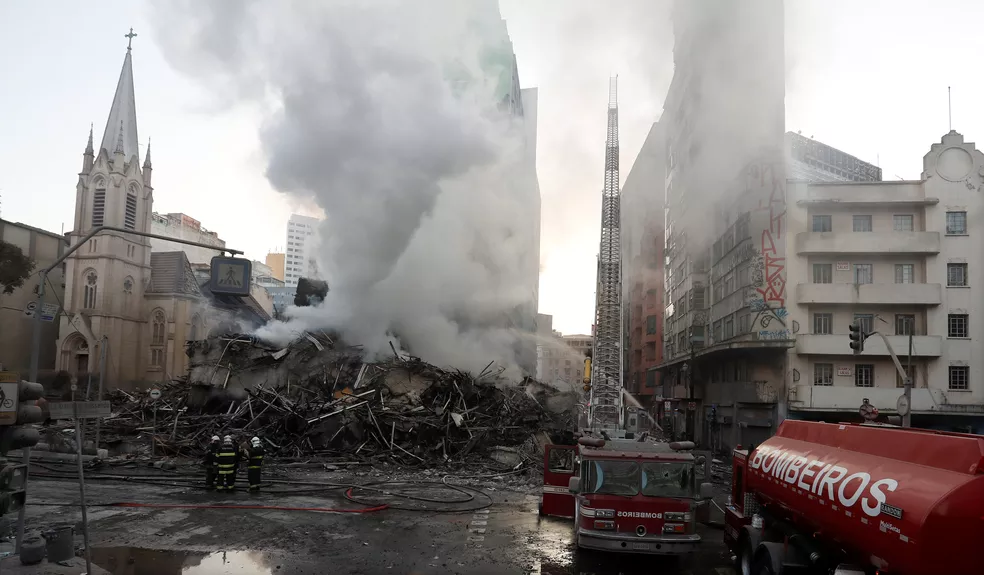
\includegraphics[width=0.8\textwidth]{paisandu.png}
  \caption{Ambiente de Trabalho \cite{sp2020}}
\end{figure}

\end{frame}

% ----------------- NOVO SLIDE --------------------------------
\section{Revisão Bibliográfica}

\begin{frame}{Revisão Bibliográfica}
\begin{itemize}
\item Operação remota de um robô SAR exige grande esforço cognitivo de dois operadores \cite{Robin2004}
\item Membros da equipe de busca e salvamento se acostumam rapidamente ao agente robótico \cite{fin2004}
\item Maior parte da comunicação é não verbal \cite{fin2004}
\item Melhoria no relacionamento homem máquina a partir de pequenas modificações \cite{habib2011}
\item A resposta SAR se alonga no tempo \cite{krui2015}
\item Capacidade de navegação autônoma \cite{tardioli2016}
\end{itemize}
\end{frame}
% ----------------- NOVO SLIDE --------------------------------
\section{Modelo}

\begin{frame}
\frametitle{Modelo}
\framesubtitle{Requisitos}
\begin{itemize}
\item O robô deverá construir mapas e se localizar no mapa construído;
\item O robô deverá operar em vários módulos: remotamente operado, semi-autônomo, autônomo;
\item O robô deverá captar sinais de áudio que sejam pistas da localização das vítimas;
\item O robô deverá reconhecer gestos simples como: siga, pare, esquerda, direita;
\item O robô deverá possuir um meio de comunicação não verbal que seja visível no ambiente da Zona Quente;
\item O robô deverá reconhecer comandos de voz simples: siga, pare, esquerda, direita;
\end{itemize}
\end{frame}
% ----------------- NOVO SLIDE --------------------------------

\begin{frame}
\frametitle{Modelo}
\framesubtitle{Aparência}
\begin{figure}
  \centering
  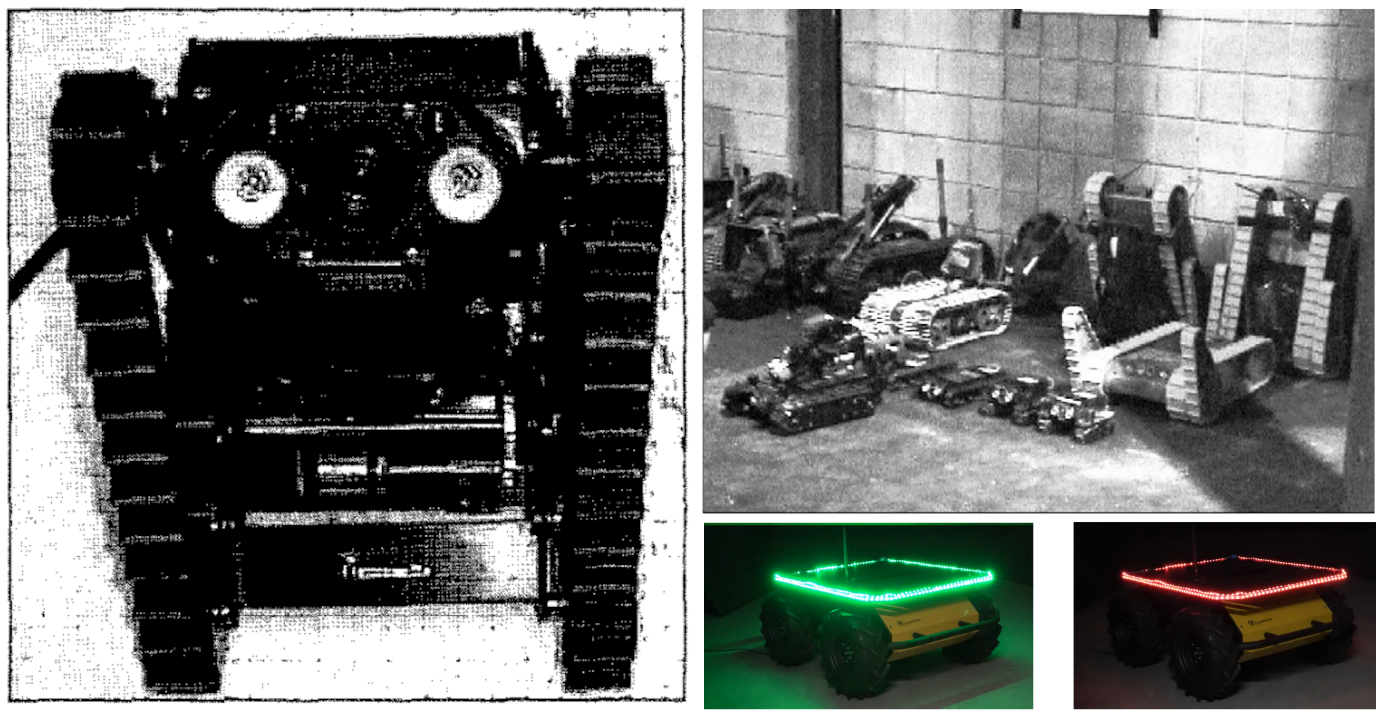
\includegraphics[width=0.8\textwidth]{robos-sar.png}
  \caption{Aparência Robô SAR}
\end{figure}


\end{frame}
% ----------------- NOVO SLIDE --------------------------------
\begin{frame}
\frametitle{Modelo}
\framesubtitle{Capacidades Sociais}
\begin{itemize}
\item Compreender gestos
\item Exibir emoções a partir da fita de led
\end{itemize}
\end{frame}
% ----------------- NOVO SLIDE --------------------------------

\begin{frame}
\frametitle{Modelo}
\framesubtitle{Área de Aplicação}
\begin{itemize}
\item Espaços confinados
\item Espaços confinados de dimensão menor que um ser humano
\end{itemize}
\end{frame}
% ----------------- NOVO SLIDE --------------------------------

\begin{frame}
\frametitle{Modelo}
\framesubtitle{Funcionalidade}
\begin{itemize}
\item Busca e Salvamento
\item Mapeamento da região
\item Descobrimento de vítimas
\end{itemize}
\end{frame}
% ----------------- NOVO SLIDE --------------------------------

\begin{frame}
\frametitle{Modelo}
\framesubtitle{Autonomia e Inteligência}
\begin{itemize}
\item Elaborar o próprio caminho
\item Desviar de obstáculos
\end{itemize}
\end{frame}
% ----------------- NOVO SLIDE --------------------------------

\begin{frame}
\frametitle{Modelo}
\framesubtitle{Consciência Situacional}
\begin{itemize}
\item Se localizar no mapa criado
\item Verificar se o avanço é possível
\item Sinalizar por ajuda
\end{itemize}
\end{frame}
% ----------------- NOVO SLIDE --------------------------------

\begin{frame}
\frametitle{Modelo}
\framesubtitle{Comportamento Temporal}
\begin{itemize}
\item A
\end{itemize}
\end{frame}
% ----------------- NOVO SLIDE --------------------------------
\section{Referências}

% --- O comando \allowframebreaks ---
% Se o conteúdo não se encaixa em um quadro, a opção allowframebreaks instrui 
% beamer para quebrá-lo automaticamente entre dois ou mais quadros,
% mantendo o frametitle do primeiro quadro (dado como argumento) e acrescentando 
% um número romano ou algo parecido na continuação.

\begin{frame}[allowframebreaks]{Referências}
\bibliography{abntex2-modelo-references}
\end{frame}

% ----------------- FIM DO DOCUMENTO -----------------------------------------
\end{document}
